\documentclass{article}
\usepackage[utf8]{inputenc}
\usepackage[a4paper, total={7in, 10in}]{geometry}
\usepackage{braket}
\usepackage{xcolor}
\usepackage{amsmath}
\usepackage{amssymb}
\usepackage{amsfonts}
\usepackage{graphicx}
\usepackage{svg}
\usepackage{float}
\usepackage{tikz}
\usepackage[ruled,vlined]{algorithm2e}
\usepackage{multicol}
\usepackage[backend=biber,style=alphabetic,sorting=ynt]{biblatex}
\usepackage{xcolor}
%\addbibresource{sample.bib} %Import the bibliography file

\newcommand{\commentt}[1]{\textcolor{blue}{ \textbf{[COMMENT]} #1}}
\newcommand{\ctt}[1]{\commentt{#1}}
\newcommand{\prb}[1]{ \mathbf{Pr} \left[ {#1} \right]}
\newcommand{\onotation}[1]{\(\mathcal{O} \left( {#1}  \right) \)}
\newcommand{\ona}[1]{\onotation{#1}}
\newcommand{\PSI}{{\ket{\psi}}}
\newcommand{\LESn}{\ket{\psi_n}}
\newcommand{\LESa}{\ket{\phi_n}}
\newcommand{\LESs}{\frac{1}{\sqrt{n}}\sum_{i}{\ket{\left(0^{i}10^{n-i}\right)^{n}}}}
\newcommand{\Hn}{\mathcal{H}_{n}}
\newcommand{\Ep}{\frac{1}{\sqrt{2^n}}\sum^{2^n}_{x}{ \ket{xx}}}
\newcommand{\HON}{\ket{\psi_{\text{honest}}}}
\newcommand{\Lemma}{\paragraph{Lemma.}}


\setlength{\columnsep}{0.6cm}

\newcommand{\Gz}{ G_{z}^{\delta} } 

\begin{document}

\title{Quantum LTC With Positive Rate}
\author{David Ponarovsky}
\maketitle
\begin{multicols*}{2}
\newcommand{ \Hw }{ \delta\Delta -\Delta^{\frac{1}{2}-\varepsilon}/\delta  }
	\newcommand{ \Nw }{ \Delta^{\frac{3}{2}-\varepsilon}} 
	  \newcommand{ \Gu } { \Gamma^{\cup} }
	  \newcommand{ \Guq } { \Gamma^{\cup, \square} }

    	\newcommand{ \Gsa } {\Gamma_{\square_{1}} }
	\newcommand{ \Gsah } { \Gamma_{\square_{1}}^{h}} 
	\newcommand{ \Gsb } {\Gamma_{\square_{2}} }
	\newcommand{ \Gsbh } {\Gamma_{\square_{2}}^{h} }
	\newcommand{ \Gssh } { \Gamma_{\square \square }^{h}}
        \newcommand{ \Aa } { C_{A_{1}}}  
	\newcommand{ \Ab } { C_{A_{2}}}
	\newcommand{ \Ac } { C_{A_{3}}}
	\newcommand{ \Ad } { C_{A_{4}}}
	\newcommand{ \Aab } { \Aa \otimes \Ab } 
	\newcommand{ \Acd } { \Ac \otimes \Ad } 
	\newcommand{ \Aac } { \Aa \otimes \Ac }
	\newcommand{ \Aabc } { \Aa \otimes \Ab \otimes \Ac }
	\newcommand{ \Aabp } { \Aa^{\perp} \otimes \Ab^{\perp} } 
	\newcommand{ \Aacp } { \Aa^{\perp} \otimes \Ac^{\perp} }
	\newcommand{ \Acdp } { \Ac^{\perp} \otimes \Ad^{\perp} }
	\newcommand{ \Aabcp } { \Aa^{\perp} \otimes \Ab^{\perp} \otimes \Ac^{\perp} }
	\newcommand{ \Aabpp } { \left( \Aabp \right)^\perp } 
	\newcommand{ \Acdpp } { \left( \Acdp \right)^\perp } 
	\newcommand{ \Aacpp } { \left( \Aacp \right)^\perp }
	\newcommand{ \Aabcpp } { \left( \Aabcp \right)^\perp }
	\newcommand{ \Aabcdpp } { \Aabpp \otimes \Acdpp  }
	\newcommand{ \YY } {  y_{1}y_{2}^{\top} }
	\newcommand{ \ZZ } {  z_{1}z_{2}^{\top} } 
	\newcommand{ \TT } { \tilde{\tau} } 


  \paragraph{preamble.} preamble.  
  \paragraph{The Construction.} Fix primes $q,p_1,p_2,p_3,p_4$ such that each of them has $1 $ residue mode $4$. Let $A_{1},A_{2},A_{3},A_{4}$ be a different generators sets of $ \mathbf{PGL}(2 , \mathbb{Z} / q\mathbb{Z} )  $ 
  obtained by taking the solutions for $a_{0}^{2} + a_{1}^{2} +a_{2}^{2} +a_{3}^{2} = p_i $ such that the pairs $A_{1},A_{2}$ and $A_{3},A_{4}$ satisfy the 
  TNC constraint and also they all satisfy that constraint togther, namly for any $g \in \mathbf{PGL}$  and $a_{1}\in A_{1}, a_{2} \in A_{2}, a_{3} \in A_{3}, a_{4} \in A_{4}$ we have that $ g \neq a_{3}a_{1}ga_{2}a_{4}$. 
  
  For any $h \in \mathbb{Z}_{3}^{2} $ define the groups $G^{h}, H^{h}$ to be: 
  \begin{equation*}
    \begin{split}
      H^{h} &=  h + \mathbb{Z}_{3}^{2}\cap \braket{ \left( 1,1 \right)} \\
      G^{h} &=  \mathbf{PGL}  \times H^{h} 
    	\end{split}
\end{equation*} 
  Then consider the graphs:   
  \begin{equation*}
    \begin{split}
      %\Gamma_{1}  &= Cay_{3}\left(  G, A_{1} \right)\times_{G} Cay_{3}\left(  G, A_{2} \right) \\
      %\Gamma_{2}  &= Cay_{3}\left(  G, A_{3} \right)\times_{G} Cay_{3}\left(  G, A_{4} \right) \\
      \Gamma_{\square_{1}}^{h} &= \bigg( G^{h}, \bigg{\{} \left( \left(g, h_{1} \right),\left(  agb,h_{1} + \left( 1,1 \right)  \right)\right) :  \\ 
      &  a \in A_{1}, b \in A_{2}, h_{1} \in H^{h}  \bigg{\}}  \bigg) \\
      \Gamma_{\square_{2}}^{h} &= \bigg( G^{h}, \bigg{\{} \left( \left(g, h_{1} \right),\left(  cgd,h_{1} + \left( 1,1 \right)  \right)\right) :  \\ 
      &  c \in A_{3}, d \in A_{4}, h_{1} \in H^{h}  \bigg{\}}  \bigg) \\
      \Gamma_{\square \square}^{h} &= \bigg( G^{h}, \bigg{\{} \left(\left(g, h_{1} \right),\left(  cagbd, h_{1} + \left( 2,2 \right)  \right)\right), \left( g, acgdb \right) :\\
      & a \in A_{1}, b \in A_{2}, c \in A_{3}, d \in A_{4}, h_{1}\in H^{h} \bigg{\}}  \bigg) 
    \end{split}
  \end{equation*}
   Then define the codes:
	\begin{equation*}
	  \begin{split}
	    C_{z}^{\perp} & = \mathcal{T}\left( \Gsah,  \Aab  \right) \\
	    & \ \ + \ \mathcal{T}\left(  \Gsbh, \Acd \right) \\
	    C_{x} &=  \mathcal{T}\left(  \Gsah, \Aabpp  \right) \\
	    & \ \ + \ \mathcal{T}\left( \Gsbh,  \Acdpp  \right) \\
	    C_{w} &=  \mathcal{T}\left( \Gssh , \Aabcdpp \right)   
	  \end{split}
	\end{equation*}
	Notice that the faces of $\Gamma_{\square_{1}},\Gamma_{\square_{2}}$ are disjointed and here the symbol $|$ means just joint them together. 
	The main focus here is to prove local test-ability for computation base (i.e $C_{x}$) and for completeness one also must to define the code 
	\begin{equation*}
	  \begin{split}
	    C_{w_{z}} &=  \mathcal{T}\left( \Gamma_{\square \square}, \left(  C_{A_1} \otimes C_{A_2} \otimes C_{A_3} \right)^{\perp}  \right)   
	  \end{split}
	\end{equation*}
	%\newcommand{}
\begin{figure}[H]
%\label{fig:square}
\begin{center}
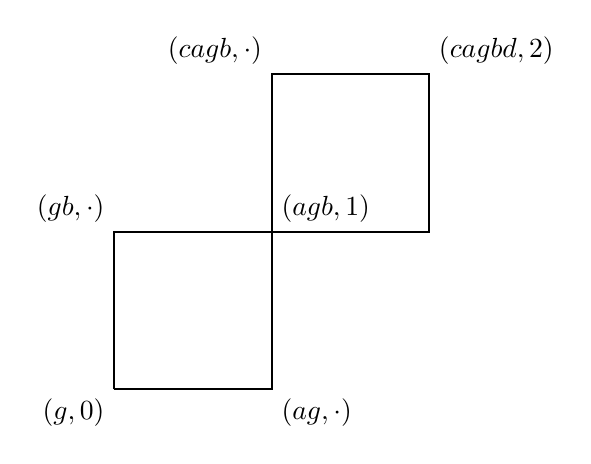
\begin{tikzpicture}
  \draw[thick] (0,0) -- (0,2) -- (2,2) -- (2,4) -- (4,4) -- (4,2) -- (2,2) -- (2,0) -- (0,0);
\node[below left] at (0,0) {$ (g,0)$};
\node[above left] at (0,2) {$ (gb,\cdot)$};
\node[above right] at (2,2) {$ (agb,1)$};
\node[below right] at (2,0) {$ (ag,\cdot)$};
\node[above left] at (2,4) {$ (cagb,\cdot)$};
\node[above right] at (4,4) {$ (cagbd,2)$};

\end{tikzpicture}
\end{center}
\caption{Square of the complex, with edges $(g,ag), (agb, gb) \in E_A,
(g,gb), (agb, ag) \in E_B.$ \label{fig:square}
}
\end{figure}

\paragraph{Lemma 1.} Fix a vertex $g$ and assume that the local views $c_1,c_2$ that lay over the graphs $\Gsa, \Gsb$ belongs to the dual tensors $\Aabpp, \Aacpp$. And inaddtion $ 1^{\Delta} \in \Aa $ then 
      \begin{equation*}
      \phi_{g}\left( c_1, c_2 \right) \in \Aabcpp
    \end{equation*}
    \paragraph{Proof.} The case where $c_{1} \in \mathbb{F}^{A_{1}} \otimes \Ab$ or $c_{2} \in \mathbb{F}^{A_{1}} \otimes \Ac $ is trival. Suppose that both $ c_{1} \in \Aa \otimes \mathbb{F}^{A_{2}}$ and $ c_{2} \in \Aa \otimes \mathbb{F}^{A_{3}}$. And consider by $h$ arbirary check of $\Aa$.Then: 
    \begin{equation*}
      \begin{split}
	\braket{h_{bc}, \phi_{g} \left( c_1, c_2 \right)  } & \ \ \ \ \ = \sum_{a}{h_{a}c_{abc}} = 
	  \sum_{a}{h_{a}c_{1_{ab}}c_{2_{ac}}} = \\ 
	  &\overset{\text{ for  } y,z\in \Aa}{\overbrace{=}}  \sum_{a} h_{a}z_{a}y_{a} \\ 
	  &\ \ \ \ \ = |h| -  \sum_{a} {h_{a} \left( \overline{ z_{a}y_{a}}  \right)} \\
	  &\ \ \ \ \ = |h| -  \sum_{a} {h_{a} \left( z_{a} + y_{a}  \right)} \\  
	  &\ \ \ \ \ = |h| +  \sum_{a} {h_{a} \left( z_{a} + y_{a}  \right)} \\ 
	  &\ \ \ \ \ =  \sum_{a} {h_{a} \left( 1^{\Delta} + z_{a} + y_{a}  \right)} 
      \end{split}
    \end{equation*}
    But $1^{\Delta} \in \Aa$ and therfore the $ \braket{h, 1^{\Delta} + z + y} = 0 $. Or in other words the words that lay over the row obtained by fixing $bc$-row is in $ C_{A_{1}}$. Hence $\phi \left( c_{1}, c_{2} \right) \in C_{A_{1}}\otimes \mathbb{F}^{A_{2}} \otimes \mathbb{F}^{A_{3}} \subset \Aabcpp$.   

    \paragraph{Lemma 2.} \textit{ Let $x \in C_{x}$ such that $ \phi(x) \in C_{w}$. And let $g$ be a negative vertex. Consider a codeword $c \in \Aabc$ then there exists $y \in C_{x}$ such that $\phi\left( x \right) + c  = \phi\left(y\right)$.   }
    \paragraph{Proof.} By definiation of the tensor code, there are codewords $v,u,w$ in $\Aa, \Ab, \Ac$ such $ c_{ijk} = v_{i}u_{j}w_{k}$. Since $v_{i} \in \mathbb{F}_{2}$ we have that
    \begin{equation*}
      \begin{split}
	 v_{i} &= v_{i}^{2} \\
	 &\Rightarrow c_{ijk}= v_{i}^{2}u_{j}w_{k}=\left( vu^{\top} \right)_{ij}\left( vw^{\top} \right)_{ik}
      \end{split}
    \end{equation*}
    define $y$ to be the addition of  $\left( vu^{\top} \right)_{ij}$ and $\left( vw^{\top} \right)_{ik}$on the $\left(A_{1},A_{2}  \right), \left(A_{1}, A_{3}\right) $ faces correspondly. 

	\paragraph{What We Currently Have.} Given a candidate for a codeword $c$ we could check efficiently if $c\in C_{z}^\perp$.  
	Additionally summing up the local correction of each vertex in $C_{x}$ yields a codeword in $C_{w}$. Now we would want to show 
	something similar to property 1 in Levarier and Zemor which imply that any codeword of $C_{w}$ with weigh beneath 
	a linear threshold $\eta n $ must to be also in $C_{X}$. (And therefore we can reject candidates with high weight). 
	%(And maybe we would also say something about the gap between the this minimal weight of $C_{w}/C_{x}$. 

	Assume that we have succeed to do so, Then the testing protocol will be looked as follow, 
	first we check that the candidate is not in $C_{z}^\perp$ and then we check that is indeed in $C_{x}$. And repeat again 
	in the phase base. Then there are constants $\kappa_1, \kappa_2$ 
	\begin{equation*}
	  \begin{split}
	    \text{accept} & \sim \kappa_1 \cdot  d\left( c,C_{z}^\perp \right)  \\ 
	    & +  \left[ 1 -  \kappa_1 \cdot  d\left( c,C_{z}^\perp \right)\right] \kappa_{2} d\left( c, C_{x} \right) \\
	    \text{reject} & \sim  \left[ 1 -  \kappa_1 \cdot  d\left( c,C_{z}^\perp \right)\right] \\ 
	    & +\kappa_1 \cdot  d\left( c,C_{z}^\perp \right) \cdot \left[ 1 - \kappa_{2} d\left( c, C_{x} \right) \right] 
	  \end{split}
	\end{equation*}
	\paragraph{Disclaimer.} The use of the $\sim$ was  made by purpose. The above should be formalize by inequalities. (And this also make another problem as 
	the term $ 1 - \kappa_{1} \cdot d\left(  \right) $ is in the opposite direction). 
	\paragraph{The Hard Part.} It seems (at least for now) that the hard part is to find an analog for Lemma 1 in Levrier-Zemor, Which can formalize 
	as follow: Consider a codeword $c \in C_{w}$ such that $|c| \le \eta n $ then we could always find a vertex in $\Gamma_{\square_{1}} $
	and a local codeword $\xi \in C_{A_1} \otimes c_{A_2} $ on his support such that $|c + \xi| < |c| $.     
      

	\paragraph{Tasks.}
	\begin{enumerate}
	  \item Prove that $\Gamma_{\square \square } $ is indeed an expander. Should be (relative) easy.
	  \item Prove a Lemma 1 analogy. And while do so, understand what are the properties we should require from the small code.
	    (i.e w-robustness and p-resistance for puncturing). 
	  \item Show that we could actually choose such $\left\{ A \right\}_{i}$ and the matched small codes.
	  \item Understand what it mean quantomlly test if a $c \in C_{w}/ C_{x}$. Namely, is weight counting can be consider as 
	    $X-$check which commute with the other $Z-$checks? 
	  \item Write a program which plot small complex in a small scale for getting more intuition. 
	\end{enumerate}
	% be a codeword with weight less then $\alpha n$.

	
	\paragraph{All The Vertices Are Normal } Define a normal vertex in $ V_{1} $ to be a vertex such his local view (a codeword in a dual tensor code). 
	supported on less then $w = \Delta^\frac{3}{2}$ faces.
	Consider the code $C_{w}$ defined above, and assume in addition that the distance and the rate of 
	the small codes $C_{A_{j}}$, $\delta \Delta$ satisfy the equation $ \left(\Delta r\right)^{4}\left(1 - \color{red}2\color{black}\delta\right) < \frac{1}{2}\delta^{3} $ and also the code $ C_{A_{1}}  $ 
      contains the word $ 1^{\Delta} $.


      Then for any $x \in C_{w}$ such that all the vertices in the induced graphs $\Gamma_{\square_{1}},\Gamma_{\square_{2}}$  by it are normal. 
	Then there exists a vertex $ g \in V_{0} $ and a local codeword $ c \in \Aabc $ supported entirely on the neighborhood of $ g $ such that: 
	$ |x + c| \le |x| $.


	\paragraph{Proof.} Let $g$ be an arbitrary vertex in $V_{0}$ we know by Leverrir and Zemor that the local views of $g$ in  $\Gamma_{\square_{1}},\Gamma_{\square_{2}}$ are $\Delta^{3/2}$ close to 
      $\Aab $ and $ \Aac $ by the $w$-robustness property. 

	So we can represent the locals views on $g$ as the following disjointed vectors, each lays on $\Gamma_{\square_1},\Gamma_{\square_2}$:
	\begin{equation*}
	  \begin{split}
	    y &= y_{1}y_{2}^{\top} + \xi_{y} \\ 
	    z &= z_{1}z_{2}^{\top} + \xi_{z}
	  \end{split}
	\end{equation*}
	such that $ y_{1}y_{2}^{\top} \in \Aab $,  $z_{1}z_{2}^{\top}\in \Aac $ and the $\xi_{y}, \xi_{z} $ are the corresponded errors of the local views from the tensor codes. 
 
	Let $ \{ y_{1}^{j}y_{2}^{i \ \top} \} ,\{ z_{1}^{j}z_{2}^{i \ \top} \}  $ be the bases for $ \Aab $ and $ \Aac $ such that $ y_{1}^{j}, z_{1}^{j} \in \Aa $ and $ y_{2}^{i} \in \Ab, z_{2}^{i} \in \Ac $.  
	And denote by $\alpha_{ij},\beta_{ij} \in \mathbb{F}_2 $ the coefficients of $\YY$ and $\ZZ$. 

	By the fact that $1^\Delta \in \Aa$ we have that for any $i,j$ the vector: 
	\begin{equation*}
	  \begin{split}
	  \bar{y_{1}}^{j}y_{2}^{i \ \top} & =  1^\Delta y_{2}^{i \ \top} \\ 
	    & + y_{1}^{j}y_{2}^{i \ \top} = \left(1^\Delta +  y_{1}^{j} \right)y_{2}^{i \ \top} \\
	    & \in \Aab
	  \end{split}
	\end{equation*}
      And by the same calculation we get also that $ \bar{z_{1}}^{j}z_{2}^{i \ \top} \in \Aac$.

      \paragraph{Claim.} Assume that $ \YY $ and $ \ZZ $ are in the  bases defined above. Let $\tau \in \mathbb{F}_{2}^{A\times B\times C} $ such that $ \tau_{abc} = \left( \YY \right)_{ab}\left( \ZZ \right)_{ac} $ then: 
      \begin{equation*}	
      d\left( \tau, \Aabc \right) \le \left( 1-\delta \right)\Delta^{3}  
      \end{equation*}
      \paragraph{Proof.} First notice that $y_{1a}y_{2b}z_{2c} $ is a valid codeword of $\Aabc$. That because that the projection obtained by 
      fixing any two coordinates yields either a zero or a codeword of one the codes.
      
      Therefore we could consider the following codeword $ \TT_{abc} = \left( y_{1a} + \bar{z}_{1a} \right)y_{2b}y_{2c} $ and bounding the distance of $\tau$ by 
      \begin{equation*}
	\begin{split}
      & d \left( \tau, \Aabc \right)  \le d \left( \tau, \TT \right) \\ 
      & = \sum_{abc}{   \left( y_{1a} + \bar{z}_{1a} \right)y_{2b}y_{2c} \oplus  \left( y_{1a}z_{1a} \right)y_{2b}y_{2c}  } \\
      & =  \sum_{abc}{   \left( y_{1a} + \bar{z}_{1a} \oplus y_{1a}z_{1a}  \right)y_{2b}y_{2c}  } \\
      & \le | \left\{ y_{1a} = 0 \text{ and }  z_{1a} = 0   \right\} | \cdot \Delta^{2} \le \left( 1-\color{red}2\color{black}\delta \right)\Delta^{3} 
	\end{split}
      \end{equation*}

      \paragraph{Claim.} Let $\YY, \ZZ$ be codewords in $\Aab, \Aac$. And let $w$ be the vector define by $w_{abc} = \left( \YY \right)_{ab} \left( \ZZ \right)_{ac} $. Then  
      \begin{equation*}
	d\left(w, \Aabc \right) \le \left( r\Delta \right)^{4}\left( 1 - \delta \right)\Delta^{3} + \Theta \left( \Delta^{2\frac{1}{2}}  \right)
      \end{equation*}

      Consider again the representation of the local view $w$ on the vertex $g$. 
      \begin{equation*}
	\begin{split}
	  & w_{abc} = y_{ab}z_{ac} = \left( \YY + \xi_{y} \right)_{ab}   \left( \ZZ + \xi_{z} \right)_{ac} \\ 
	  & \left( y_{1}y_{2}^{\top}\right)_{ab}\left(z_{1}z_{2}^{\top} \right)_{ac} = 
	  \left( \sum_{ij} { \alpha_{ij} y_{1}^{i}y_{2}^{j  \top}}  \right)_{ab}\left(   \sum_{ij} { \beta_{ij} z_{1}^{i}z_{2}^{j  \top}} \right)_{ac}\\ 
	  &= \sum_{ijlk} { \alpha_{ij}\beta_{lk} y_{1a}^{i}y_{2b}^{j \top}} z_{1a}^{l}z_{2c}^{k \top} \\
	  & \Rightarrow d\left( \sum_{abc} \left( y_{1}y_{2}^{\top}\right)_{ab}\left(z_{1}z_{2}^{\top} \right)_{ac} , \Aabc \right) \\ 
	  & \ \ \ \ \le \left( \Delta r \right)^{4} \left( 1-\delta \right)\Delta^{3} \\ & 
	  %+  \left( \xi_{y} z_{1}z_{2}^\top + \xi_{y}\xi_{z}, \Aabc   \right)  
	\end{split}
      \end{equation*}
      In addition its clear that $ | \sum_{abc}{\xi_{ab}\left( \ZZ + \xi\right)_{ac}} | \le  \sum_{c}\sum_{ab}{|\xi_{ab}|} \le \Delta^{ 2\frac{1}{2}} $. Hence, we have that 
  \begin{equation*}
    \begin{split}
      d\left( w, \Aabc  \right) \le  \left( r\Delta \right)^{4}\left( 1 - \delta \right)\Delta^{3} + \Theta \left( \Delta^{2\frac{1}{2}}  \right)
    \end{split}
  \end{equation*}
  		\paragraph{Dense Normal Net Counting} Let us call the normal vertices the vertices with degree less then $\xi$ in $\Guq = \Gamma_{\square, 1}^{x} \cup \Gamma_{\square, 2}^{x}$. 
    And Let us say that that an edge of $\Gu$ is heavy if it is incident to at least $\eta$ squares in $\Gsa$ and $\Gsb$. Let $ T$ be set of vertices in $V_0$ that are connected to (at least) one normal vertex through a heavy edge. 

    First notice that the number of vertices in the induced graph by $x$ is bounded by it's weight:
    $ |S| \le \frac{2|x|}{ \delta\Delta }$ 

    By the mixing Lemma we get:  
    \begin{equation*}
      \begin{split}
	|E\left( S,T \right)| & \ge \eta |T| \\ 
	|E\left( S,T \right)| & = |E\left( S,T \right)_{\Gamma_{1}} \cup E\left( S,T \right)_{\Gamma_{2}} | \\ 
      \le & \frac{|S||T|}{n}\left( 2 \cdot 2\Delta - \Delta  \right) \\ & + \sqrt{|S||T|}\left( 2\cdot \lambda_{ \text{double cover} } + \lambda_{ \text{ramnujan} }    \right)
      \end{split}
    \end{equation*}
    Hence we have that:
    \begin{equation*}
      \begin{split}
	& |T|\left( \eta - \frac{2|x|}{\delta\Delta}\cdot\frac{3\Delta}{n}  \right)\le \sqrt{|S||T|}\lambda^{\star} \\ 
	& |T| \le \left(\frac{\lambda^{\star}}{\eta - \frac{6|x|}{n \delta}}\right)^{2}|S|
      \end{split}
    \end{equation*}
    Denote by $S_{e}$ the set of vertices in $\Guq$ with degree greater then $\xi$. Then by repeating on the above calculation, while substituting $\Gamma_{i}$ by $\Gamma_{i, \square}$, We obtain that there is $\lambda^{\star}_{2}$ such that:
     \begin{equation*}
      \begin{split}
	& |S_{e}| \le \left(\frac{\lambda^{\star}_{2}}{\xi - \left(2\Delta^{2} - \Delta  \right)\frac{|x|}{n \delta\Delta}}\right)^{2}|S|
      \end{split}
    \end{equation*}
    Define $\bar{d}_{T}$ to be the average (over $T$) of heavy edges incident to a vertex of $T$. So 
    \begin{equation*}
      \begin{split}
	\bar{d}_{T} &= \frac{|E\left( T, S / S_{e} \right)|}{T} \ge \frac{|S| - |S_{e}|}{|T|} \\
	& \ge \left( 1 -   \left(\frac{\lambda^{\star}_{2}}{\xi - \left(2\Delta^{2} - \Delta  \right)\frac{|x|}{n \delta\Delta}}\right)^{2}\right) /  
	  \left(\frac{\lambda^{\star}}{\eta - \frac{6|x|}{n \delta}}\right)^{2}
      \end{split}
    \end{equation*}
    Let us call to the quantity above $\Delta\rho$ and denote by $1 - \tau$ the fraction of vertices of $ T $ with degree less then $\frac{1}{2}\Delta\rho$. 
 Then $ \Delta\rho \le \bar{d}_{T} \le 3\Delta\tau + \left( 1 - \tau \right) \Delta\rho  $ 
 $ \Rightarrow \tau \ge \frac{\rho}{2\left( 3 - \rho \right)}\ge \rho/3 $. Namely, at least $\rho/3$ of vertices of $T$ are incident to at least $\frac{1}{2}\Delta\rho$ heavy edges. 

 Since $\Gu$ is $3\Delta$ regular we get that $|S| - |S_{e}| \le 3\Delta |T| $. In the other-hand we have shown that 
 \begin{equation*}
   \begin{split}
     |S_{e}| & \le \left(\frac{\lambda^{\star}_{2}}{\xi - \left(2\Delta^{2} - \Delta  \right)\frac{|x|}{n \delta\Delta}}\right)^{2}|S| \\ &
     \Rightarrow |S| \le \left( 1 - \left(\frac{\lambda^{\star}_{2}}{\xi - \left(2\Delta^{2} - \Delta  \right)\frac{|x|}{n \delta\Delta}}\right)^{2}\right)^{-1}3\Delta|T| \\
     & = \left( 1 - \theta^2 \right) 3 \Delta |T|
   \end{split}
 \end{equation*}
 And by using again the mixing Lemma we have that: 
 \begin{equation*}
   \begin{split}
     E\left( S_{e},T \right) &\le \frac{\theta^2}{1- \theta^2}3\Delta|T|^2 \frac{3\Delta}{n} + \lambda^{\star}\sqrt{\frac{\theta^2}{1- \theta^2}}|T| \\ 
     & \le  \left( \frac{\theta^2}{1- \theta^2}9\Delta^{2} + \lambda^{\star}\sqrt{\frac{\theta^2}{1- \theta^2}}\right)|T| \\ 
     & \le \left(9\Delta^{2} + \lambda^{\star} \right) |T|
  \end{split}
 \end{equation*}
 Hence at most an $\frac{1}{6}\rho $ proportion of vertices of $T$ are adjacent to more than $\frac{6}{\rho} \left( 9\Delta^{2} + \lambda^{\star}  \right) $ vertices of $S_{e}$, And at least $\frac{5}{6}\rho$ proportion of $T$ are adjacent to less then $\frac{6}{\rho} \left( 9\Delta^{2} + \lambda^{\star}  \right) $ . 
 And therefore we have that at least $\frac{1}{6}\rho$ vertices are:
 \begin{enumerate}
   \item Incident to at least $\frac{1}{2}\Delta\rho$ heavy edges. 
   \item Adjacent to at most $ \frac{6}{\rho} \left( 9\Delta^{2} + \lambda^{\star}  \right)$ vertices of $S_{e}$.  
 \end{enumerate}
 \paragraph{Proof Of Theorem 1} Let us call to the set of vertices satisfy the constraints above \textbf{good vertices}. Pick any good vertex $g \in T$.
 Remember that each heavy edge between a normal vertex of $S$ and a vertex of $T$ corresponds to either a row or a column shared by the two local views.
 

 By $w$-robustness, for any small enough $\xi \le w $, the local view of any normal vertex is supported on at most $\frac{\xi}{\delta\Delta}$ rows and columns. 
 Hence, the row (or column) shared between the normal vertex and $v$ is at distance at most $\frac{\xi}{\delta\Delta}$ from a nonzero codeword of $\Aa$ (or $\Ab$, $\Ac$).


 Let us denote by $x_{v^{\prime}}$ the the local view obtained by taking only the rows and columns that shared between $v$ and normal vertices. The $\gamma$-resistance to puncturing property implies that if we could find $ \eta, \xi  $ such that for any $ |x| \le d $ we have:
 \begin{equation*}
   \begin{split}
     &  \frac{6}{\rho} \left( 9\Delta^{2} + \lambda^{\star}  \right) \le \gamma \ \ \ \ \ \left( \Theta\left(  \Delta^{\frac{1}{2}} \right) \right)
   \end{split}
 \end{equation*}
 Then the local view of $v$ is at distance at most:
 \begin{equation*}
   \begin{split}
     & d\left(x_{v}, \Aabc\right) \\ 
     & \ \ \ \ \le d\left(x_{v^{\prime} }, \cdot \right) + |\text{ ignored bits }|\\
     & \ \ \ \ \le  d\left(x_{v^{\prime}}, \cdot \right) +  \color{red}\frac{3}{2} \color{black} \Delta^{\color{red} 2 \color{black} } \cdot \frac{6}{\rho} \left( 9\Delta^{2} + \lambda^{\star}  \right) 
   \end{split}
 \end{equation*}
 Choosing $ \eta, \xi, \delta, \gamma, w, |x| < d $ such that the above is lower than $\frac{1}{2}\left( \delta\Delta \right)^{3}$ finishes the proof. 
 \paragraph{Theorem 2.} \textit{ The code $C_{w} / \mathcal{T}\left( \Gamma_{\square \square}, \left(  C_{A_1} \otimes C_{A_2} \otimes C_{A_3} \right)  \right)  $ has positive rate and linear distance.}
 \paragraph{Theorem 3.} \textit{ The code defined by $C_{x}$ has an efficient test for rejecting candidate with high error weigh. } 
 \paragraph{The Decoder.} Let $x$ be a canidate that might or might not be in $C_{x}$. The decoder $\mathcal{D}$ describe below return a valid codeword of $C_{X}$ if $x$ is at distance at most $\tilde{\alpha}$ from $C_{x}$ and otherwise reject.
 First, for every positive (left) vertex $g\in G\times \mathbb{Z}_2 $,  $\mathcal{D}$ compute the codeword of the dual tensor code which is the closest to its local view. Denote each that codeword by $c_g$. 
 Then define the mismatch to be $z = \sum_{g \in G}{c_g} $ and notice that by the fact that each face is summed up twice $|z|$ eqaul the number of disagrements. 
 
 If $|z|$ is indeed zero, then $\tilde{z}$ which define by taking the ``AND'' of local correction instead of xoring them is a valid codeword. 
 $\mathcal{D}$ will defined to returns $\tilde{z}$ in that case. 

 Assume that $|z| > 0 $. Then $\mathcal{D}$ will:
 \begin{enumerate}
   \item Compute for every negative vertex the closest local view correspond to $\phi_{g}^{\perp}$. Call it, $\omega_{g}$.
   \item Sum the $\omega's$. And set the yilded bits on the plaquettes. Denote the word obtained by that by $J$.


   %\item Sum the $\omega$'s divded by $\color{red}\frac{1}{3}\color{black}$. Namly $\sum_{g\in G}{\frac{1}{3}\omega_g}$. And set the yilded bits on the plaquettes.  
   %\item Map the plaquettes values which are fractions ( $\left\{ \frac{1}{3}, \frac{2}{3} \right\}$ ) to $1$ and to $0$ otherwise. Denote the word obtained by that by $J$.
 \end{enumerate}
 Clearly $J \in C_{w}$. Denote by $e$ the error, i.e $e + x \in C_{x}$. Let us decompose  
 
 \begin{figure}[H]
            %\label{fig:square}
            \begin{center}
            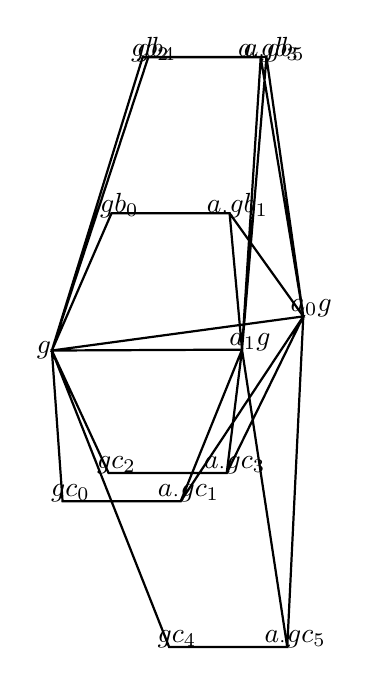
\begin{tikzpicture}
            \draw[thick](0,0)(0,0)  -- (0.7573585869902781, 1.742410894656945) -- (2.257358586990278, 1.742410894656945) -- (3.1932836010261725,0.43319882990656383) -- (0,0) -- (0,0)  -- (0.13593530800772835, -1.9155990981234063) -- (1.6359353080077284, -1.9155990981234063) -- (3.1932836010261725,0.43319882990656383) -- (0,0) -- 
(0,0)  -- (0.7573585869902781, 1.742410894656945) -- (2.257358586990278, 1.742410894656945) -- (3.1932836010261725,0.43319882990656383) -- (0,0) -- (0,0)  -- (0.7204804010709267, -1.5563780539935632) -- (2.220480401070927, -1.5563780539935632) -- (3.1932836010261725,0.43319882990656383) -- (0,0) -- 
(0,0)  -- (0.7573585869902781, 1.742410894656945) -- (2.257358586990278, 1.742410894656945) -- (3.1932836010261725,0.43319882990656383) -- (0,0) -- (0,0)  -- (1.48928186251678, -3.7659346992953777) -- (2.98928186251678, -3.7659346992953777) -- (3.1932836010261725,0.43319882990656383) -- (0,0) -- 
(0,0)  -- (1.152436218450279, 3.7238867270593956) -- (2.652436218450279, 3.7238867270593956) -- (3.1932836010261725,0.43319882990656383) -- (0,0) -- (0,0)  -- (0.13593530800772835, -1.9155990981234063) -- (1.6359353080077284, -1.9155990981234063) -- (3.1932836010261725,0.43319882990656383) -- (0,0) -- 
(0,0)  -- (1.152436218450279, 3.7238867270593956) -- (2.652436218450279, 3.7238867270593956) -- (3.1932836010261725,0.43319882990656383) -- (0,0) -- (0,0)  -- (0.7204804010709267, -1.5563780539935632) -- (2.220480401070927, -1.5563780539935632) -- (3.1932836010261725,0.43319882990656383) -- (0,0) -- 
(0,0)  -- (1.152436218450279, 3.7238867270593956) -- (2.652436218450279, 3.7238867270593956) -- (3.1932836010261725,0.43319882990656383) -- (0,0) -- (0,0)  -- (1.48928186251678, -3.7659346992953777) -- (2.98928186251678, -3.7659346992953777) -- (3.1932836010261725,0.43319882990656383) -- (0,0) -- 
(0,0)  -- (1.2250714320503318, 3.7266645458596797) -- (2.7250714320503318, 3.7266645458596797) -- (3.1932836010261725,0.43319882990656383) -- (0,0) -- (0,0)  -- (0.13593530800772835, -1.9155990981234063) -- (1.6359353080077284, -1.9155990981234063) -- (3.1932836010261725,0.43319882990656383) -- (0,0) -- 
(0,0)  -- (1.2250714320503318, 3.7266645458596797) -- (2.7250714320503318, 3.7266645458596797) -- (3.1932836010261725,0.43319882990656383) -- (0,0) -- (0,0)  -- (0.7204804010709267, -1.5563780539935632) -- (2.220480401070927, -1.5563780539935632) -- (3.1932836010261725,0.43319882990656383) -- (0,0) -- 
(0,0)  -- (1.2250714320503318, 3.7266645458596797) -- (2.7250714320503318, 3.7266645458596797) -- (3.1932836010261725,0.43319882990656383) -- (0,0) -- (0,0)  -- (1.48928186251678, -3.7659346992953777) -- (2.98928186251678, -3.7659346992953777) -- (3.1932836010261725,0.43319882990656383) -- (0,0) -- 
(0,0)  -- (0.7573585869902781, 1.742410894656945) -- (2.257358586990278, 1.742410894656945) -- (2.4148790983708883,0.011115604095153707) -- (0,0) -- (0,0)  -- (0.13593530800772835, -1.9155990981234063) -- (1.6359353080077284, -1.9155990981234063) -- (2.4148790983708883,0.011115604095153707) -- (0,0) -- 
(0,0)  -- (0.7573585869902781, 1.742410894656945) -- (2.257358586990278, 1.742410894656945) -- (2.4148790983708883,0.011115604095153707) -- (0,0) -- (0,0)  -- (0.7204804010709267, -1.5563780539935632) -- (2.220480401070927, -1.5563780539935632) -- (2.4148790983708883,0.011115604095153707) -- (0,0) -- 
(0,0)  -- (0.7573585869902781, 1.742410894656945) -- (2.257358586990278, 1.742410894656945) -- (2.4148790983708883,0.011115604095153707) -- (0,0) -- (0,0)  -- (1.48928186251678, -3.7659346992953777) -- (2.98928186251678, -3.7659346992953777) -- (2.4148790983708883,0.011115604095153707) -- (0,0) -- 
(0,0)  -- (1.152436218450279, 3.7238867270593956) -- (2.652436218450279, 3.7238867270593956) -- (2.4148790983708883,0.011115604095153707) -- (0,0) -- (0,0)  -- (0.13593530800772835, -1.9155990981234063) -- (1.6359353080077284, -1.9155990981234063) -- (2.4148790983708883,0.011115604095153707) -- (0,0) -- 
(0,0)  -- (1.152436218450279, 3.7238867270593956) -- (2.652436218450279, 3.7238867270593956) -- (2.4148790983708883,0.011115604095153707) -- (0,0) -- (0,0)  -- (0.7204804010709267, -1.5563780539935632) -- (2.220480401070927, -1.5563780539935632) -- (2.4148790983708883,0.011115604095153707) -- (0,0) -- 
(0,0)  -- (1.152436218450279, 3.7238867270593956) -- (2.652436218450279, 3.7238867270593956) -- (2.4148790983708883,0.011115604095153707) -- (0,0) -- (0,0)  -- (1.48928186251678, -3.7659346992953777) -- (2.98928186251678, -3.7659346992953777) -- (2.4148790983708883,0.011115604095153707) -- (0,0) -- 
(0,0)  -- (1.2250714320503318, 3.7266645458596797) -- (2.7250714320503318, 3.7266645458596797) -- (2.4148790983708883,0.011115604095153707) -- (0,0) -- (0,0)  -- (0.13593530800772835, -1.9155990981234063) -- (1.6359353080077284, -1.9155990981234063) -- (2.4148790983708883,0.011115604095153707) -- (0,0) -- 
(0,0)  -- (1.2250714320503318, 3.7266645458596797) -- (2.7250714320503318, 3.7266645458596797) -- (2.4148790983708883,0.011115604095153707) -- (0,0) -- (0,0)  -- (0.7204804010709267, -1.5563780539935632) -- (2.220480401070927, -1.5563780539935632) -- (2.4148790983708883,0.011115604095153707) -- (0,0) -- 
(0,0)  -- (1.2250714320503318, 3.7266645458596797) -- (2.7250714320503318, 3.7266645458596797) -- (2.4148790983708883,0.011115604095153707) -- (0,0) -- (0,0)  -- (1.48928186251678, -3.7659346992953777) -- (2.98928186251678, -3.7659346992953777) -- (2.4148790983708883,0.011115604095153707) -- (0,0) -- 
(0,0);
\node at (-0.1,0) {$ g $};
\node at (3.2932836010261726,0.5331988299065639) {$ a_{ 0 }g $};
\node at (2.5148790983708884,0.11111560409515371) {$ a_{ 1 }g $};
\node at (0.8573585869902781,1.842410894656945) {$ gb_{ 0 } $};
\node at (2.3573585869902782,1.842410894656945) {$ a_{\cdot} gb_{ 1 } $};
\node at (1.252436218450279,3.8238867270593957) {$ gb_{ 2 } $};
\node at (2.752436218450279,3.8238867270593957) {$ a_{\cdot} gb_{ 3 } $};
\node at (1.3250714320503318,3.8266645458596797) {$ gb_{ 4 } $};
\node at (2.825071432050332,3.8266645458596797) {$ a_{\cdot} gb_{ 5 } $};
\node at (0.23593530800772836,-1.8155990981234063) {$ gc_{ 0 } $};
\node at (1.7359353080077284,-1.8155990981234063) {$ a_{\cdot} gc_{ 1 } $};
\node at (0.8204804010709267,-1.4563780539935631) {$ gc_{ 2 } $};
\node at (2.320480401070927,-1.4563780539935631) {$ a_{\cdot} gc_{ 3 } $};
\node at (1.5892818625167802,-3.6659346992953776) {$ gc_{ 4 } $};
\node at (3.08928186251678,-3.6659346992953776) {$ a_{\cdot} gc_{ 5 } $};

            \end{tikzpicture}
            \end{center}
            \caption{Square of the complex, with edges $(g,ag), (agb, gb) \in E_A,
            (g,gb), (agb, ag) \in E_B.$ \label{fig:square}
            }
            \end{figure}

\end{multicols*}
  % \printbibliography 
\end{document}


